\documentclass[xcolor=dvipsnames]{beamer}

% For more themes, color themes and font themes, see:
% http://deic.uab.es/~iblanes/beamer_gallery/index_by_theme.html

\mode<presentation>
{
  \usetheme{Boadilla}      
  \usecolortheme{default} 
  \usefonttheme{default} 
  \setbeamertemplate{navigation symbols}{}
  \setbeamertemplate{caption}[numbered]
} 

\usepackage[english]{babel}
\usepackage[utf8x]{inputenc}

\usepackage{xcolor}
\usepackage{color}
\definecolor{rscuro}{rgb}{0.75,0.0,0.0}
\definecolor{bscuro}{rgb}{0.0,0.2,0.5}

\usepackage{graphicx}
\graphicspath{{Presentation_images/}}                 									   % percorso immagini
\usepackage[font=small,format=hang]{caption}  										% didascalie e numero 
\captionsetup{tableposition=top,figureposition=bottom,font=small, format=hang,labelfont={sf,bf}} 	% altre opzioni	
\usepackage{epstopdf}
\usepackage{subfig}

\title[Topics in Statistical learning]{}
\author{L. Insolia, J. Kim and Y. Yeghikyan}
\institute{SNS}
\date{March 9, 2018}

\begin{document}
	
	\begin{frame}
		\vskip 1.5cm 	
 		\centering\huge\textcolor{bscuro}{Study of French labour market and inequalities} \\
		\vskip 0.5cm 
			\centering\small \textcolor{rscuro}{--- \emph{Midterm results} ---}
			\maketitle
	\end{frame}
	
	%\begin{frame}{Outline}
	%\tableofcontents
	%\end{frame}
	
	
\section{Motivation}
		\begin{frame}{\vskip 0.05cm\centerline{\Huge\textcolor{bscuro}{Motivation}}}
%	   What were the aims of your project, and what is the context – in terms of subject matter questions, and in terms of applicable statistical and computational tools.  		
			Objective:
			\begin{itemize}
			 	 \item To study the structure of French labour market 
			 	 \item Inequalities (in terms of salary): 
			 	 \begin{itemize}
			 	 	\item ages 
			 	 	\item gender
			 	 	\item job categories
			 	 \end{itemize}
			\end{itemize}
			\vskip 1cm
\end{frame}
	
	
\section{Methodology}
		\begin{frame}{\vskip 0.05cm\centerline{\Huge\textcolor{bscuro}{Methodology}}}
%	  Description of the dataset (where is it from what is the information shared through this dataset, what year)and the variables that we have, what are the interesting features that we can use to study 
 		\begin{itemize}
			\item INSEE 
				\begin{itemize}
				\item Population; cohabitation mode, age and sex
				\item Salary; job categories, age and sex (mean net salary per hour)
				\item Firms; number and size of firms
				\item Geography; GPS latitude and longitutde
				\end{itemize}
		for different geographical levels (communes, departments, \underline{towns}) in 2014
		\end{itemize}				
\end{frame}
	
	
\section{1. What has been done so far...}
		\begin{frame}{\vskip 0.05cm\centerline{\Huge\textcolor{bscuro}{What has been done so far \ldots}}}
%	  State clearly what you were able to accomplish during the course, illustrate methods used and results.
		\begin{itemize}
		\item Population: 
					\begin{itemize}
						\item insight to demographic profile for each town 
						\item age into three different categories; child, workforce and elderly
						\item sex and dependency ratios 
					\end{itemize}
		\end{itemize}
\end{frame}


\section{1. Graphes}
		\begin{frame}
		Fig.~\ref{fig1} shows 
			\begin{figure}[!ht] 
				\centering
				\subfloat[]{{\includegraphics[width=5.5cm]{dis_pop_dep.jpeg} }}
				\qquad
				\subfloat[]{{\includegraphics[width=5.5cm]{pyramid_pop.jpeg} }}
				\caption{} 
				\label{fig1}
			\end{figure}
		\end{frame}


\section{2. What has been done so far...}
\begin{frame}{\vskip 0.05cm\centerline{\Huge\textcolor{bscuro}{What has been done so far \ldots}}}
%	  State clearly what you were able to accomplish during the course, illustrate methods used and results.
\begin{itemize}
	\item Salary:
	\begin{itemize}
		\item salary levels across different towns
		\item comparison for different job positions/ gender/ age
		\item predictions of 
	\end{itemize}
\end{itemize}
\end{frame}


\section{2. Graphes}
	\begin{frame}
		Fig.~\ref{fig2} shows 
		\begin{figure}[!ht] 
			\centering
			\subfloat[]{\includegraphics[width=0.5\textwidth]{boxplot_sex_age.jpeg}}
			\subfloat[]{\includegraphics[width=0.5\textwidth]{boxplot_sex_job.jpeg}}
			\caption{} 
			\label{fig2}
		\end{figure}
\end{frame}


\section{2.1 Graphes}
\begin{frame}
Fig.~\ref{fig3} shows 
\begin{figure}[!ht] 
	\centering
	\subfloat[]{\includegraphics[width=0.5\textwidth]{boxplot_sex_job.jpeg}}
	\caption{} 
	\label{fig3}
\end{figure}
\end{frame}


\section{3. What has been done so far...}
\begin{frame}{\vskip 0.05cm\centerline{\Huge\textcolor{bscuro}{What has been done so far \ldots}}}
%	  State clearly what you were able to accomplish during the course, illustrate methods used and results.
\begin{itemize}
	\item Firms:
	\begin{itemize}
		\item distribution of firms per town;
		\item analysis
	\end{itemize}
\end{itemize}
\end{frame}



\section{3. Graphes}
	\begin{frame}
			Fig.~\ref{} shows 
			\begin{figure}[!ht] 
				\centering
				\subfloat[]{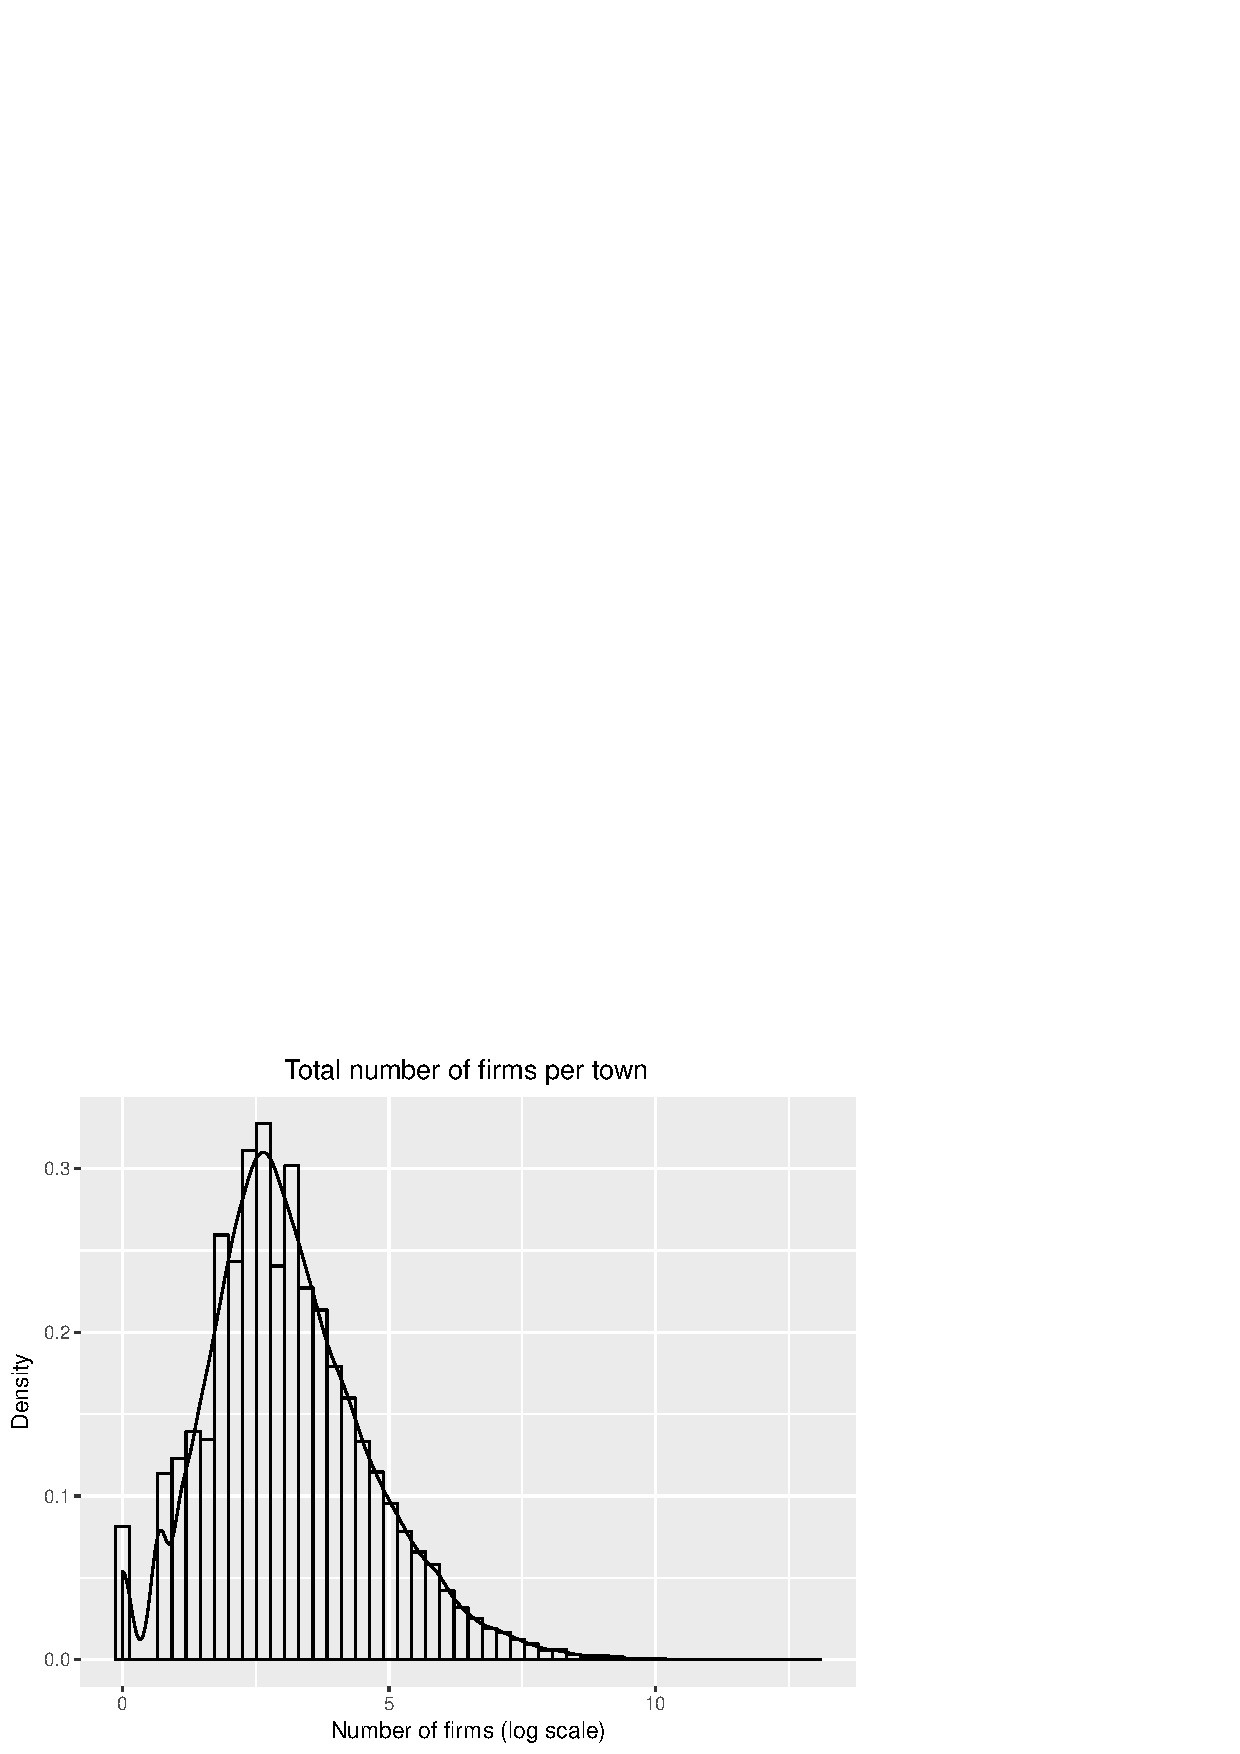
\includegraphics[width=0.5\textwidth]{hist_firms_total.jpeg}}
				\subfloat[]{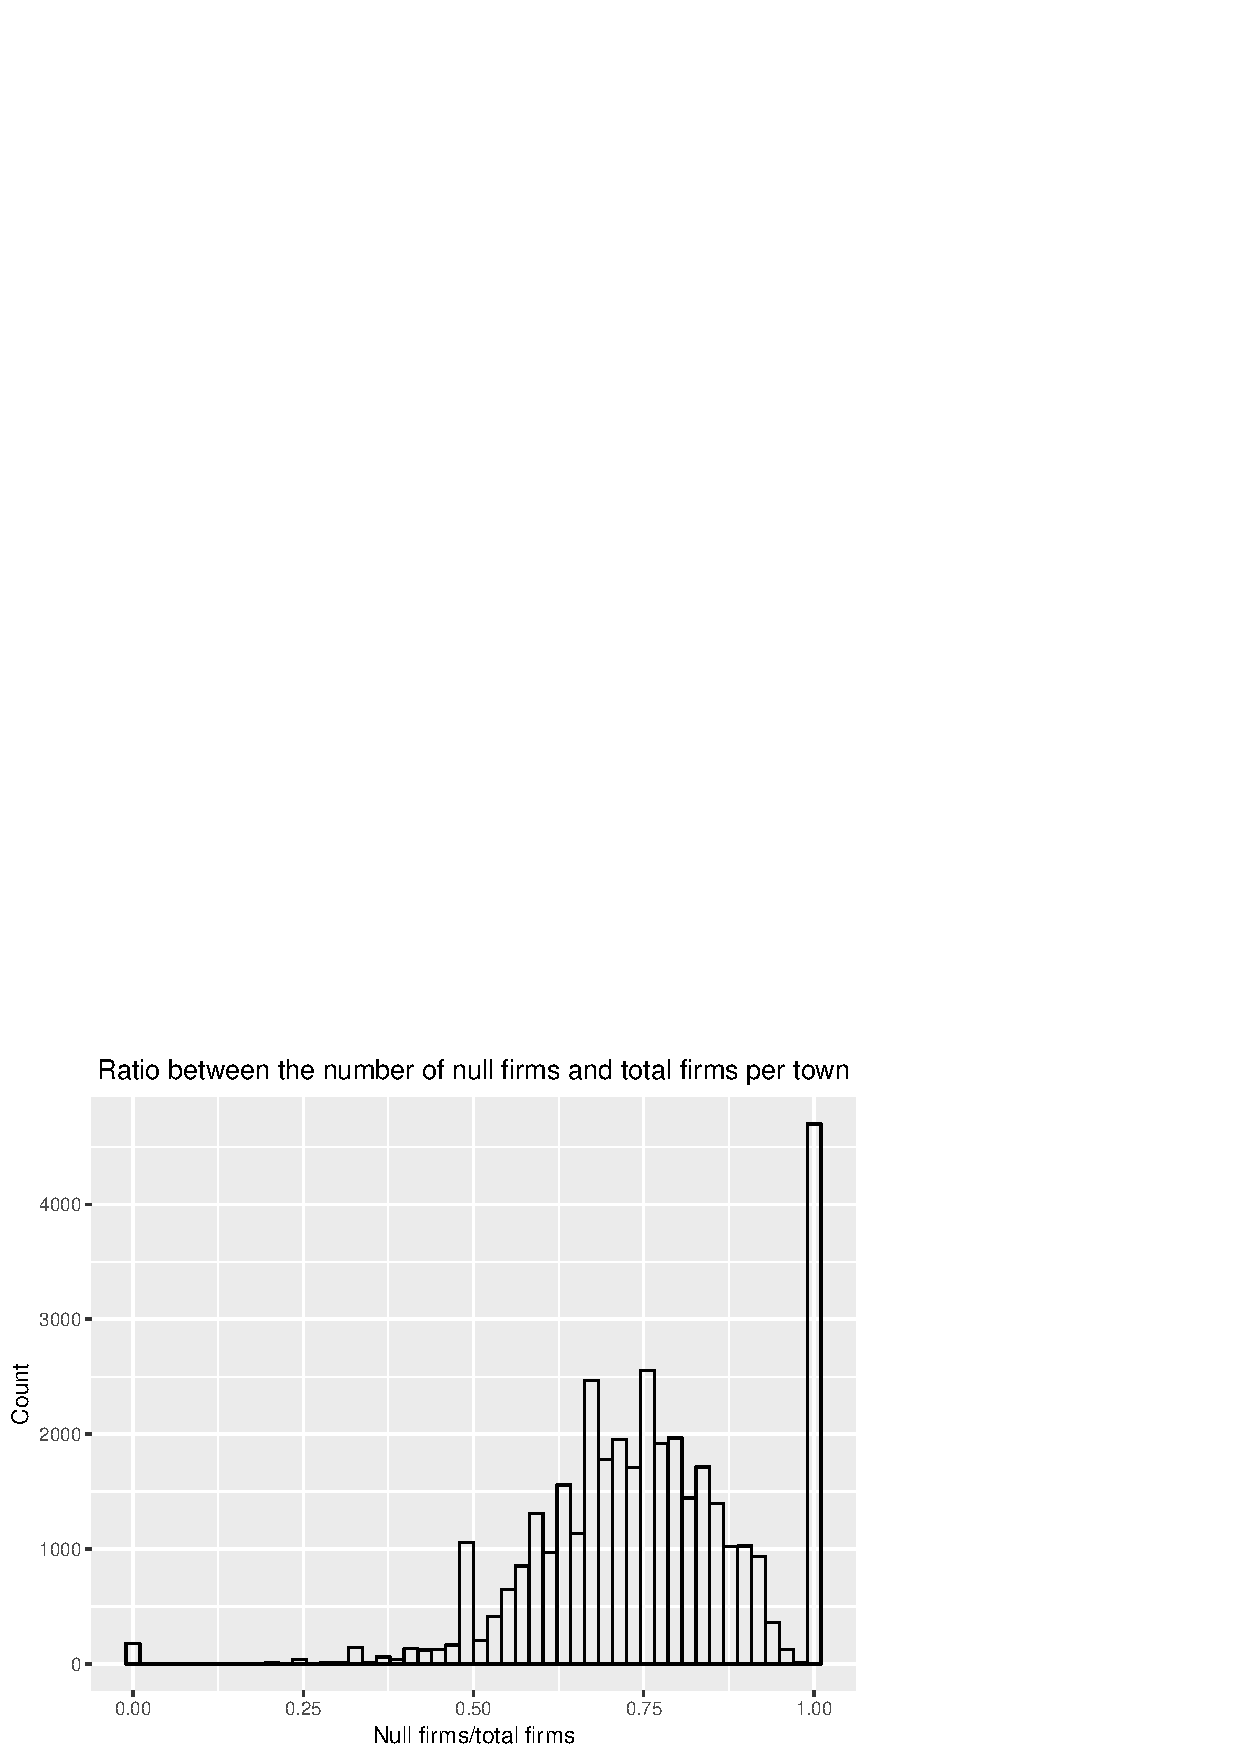
\includegraphics[width=0.5\textwidth]{hist_firms_ratio_null_total.jpeg}}
				\caption{} 
				\label{}
			\end{figure}
\end{frame}


\section{3.1 Graphes}
\begin{frame}
Fig.~\ref{fig4} shows 
\begin{figure}[!ht] 
	\centering
	\subfloat[]{\includegraphics[width=0.5\textwidth]{biplot_firms.jpeg}}
	\subfloat[]{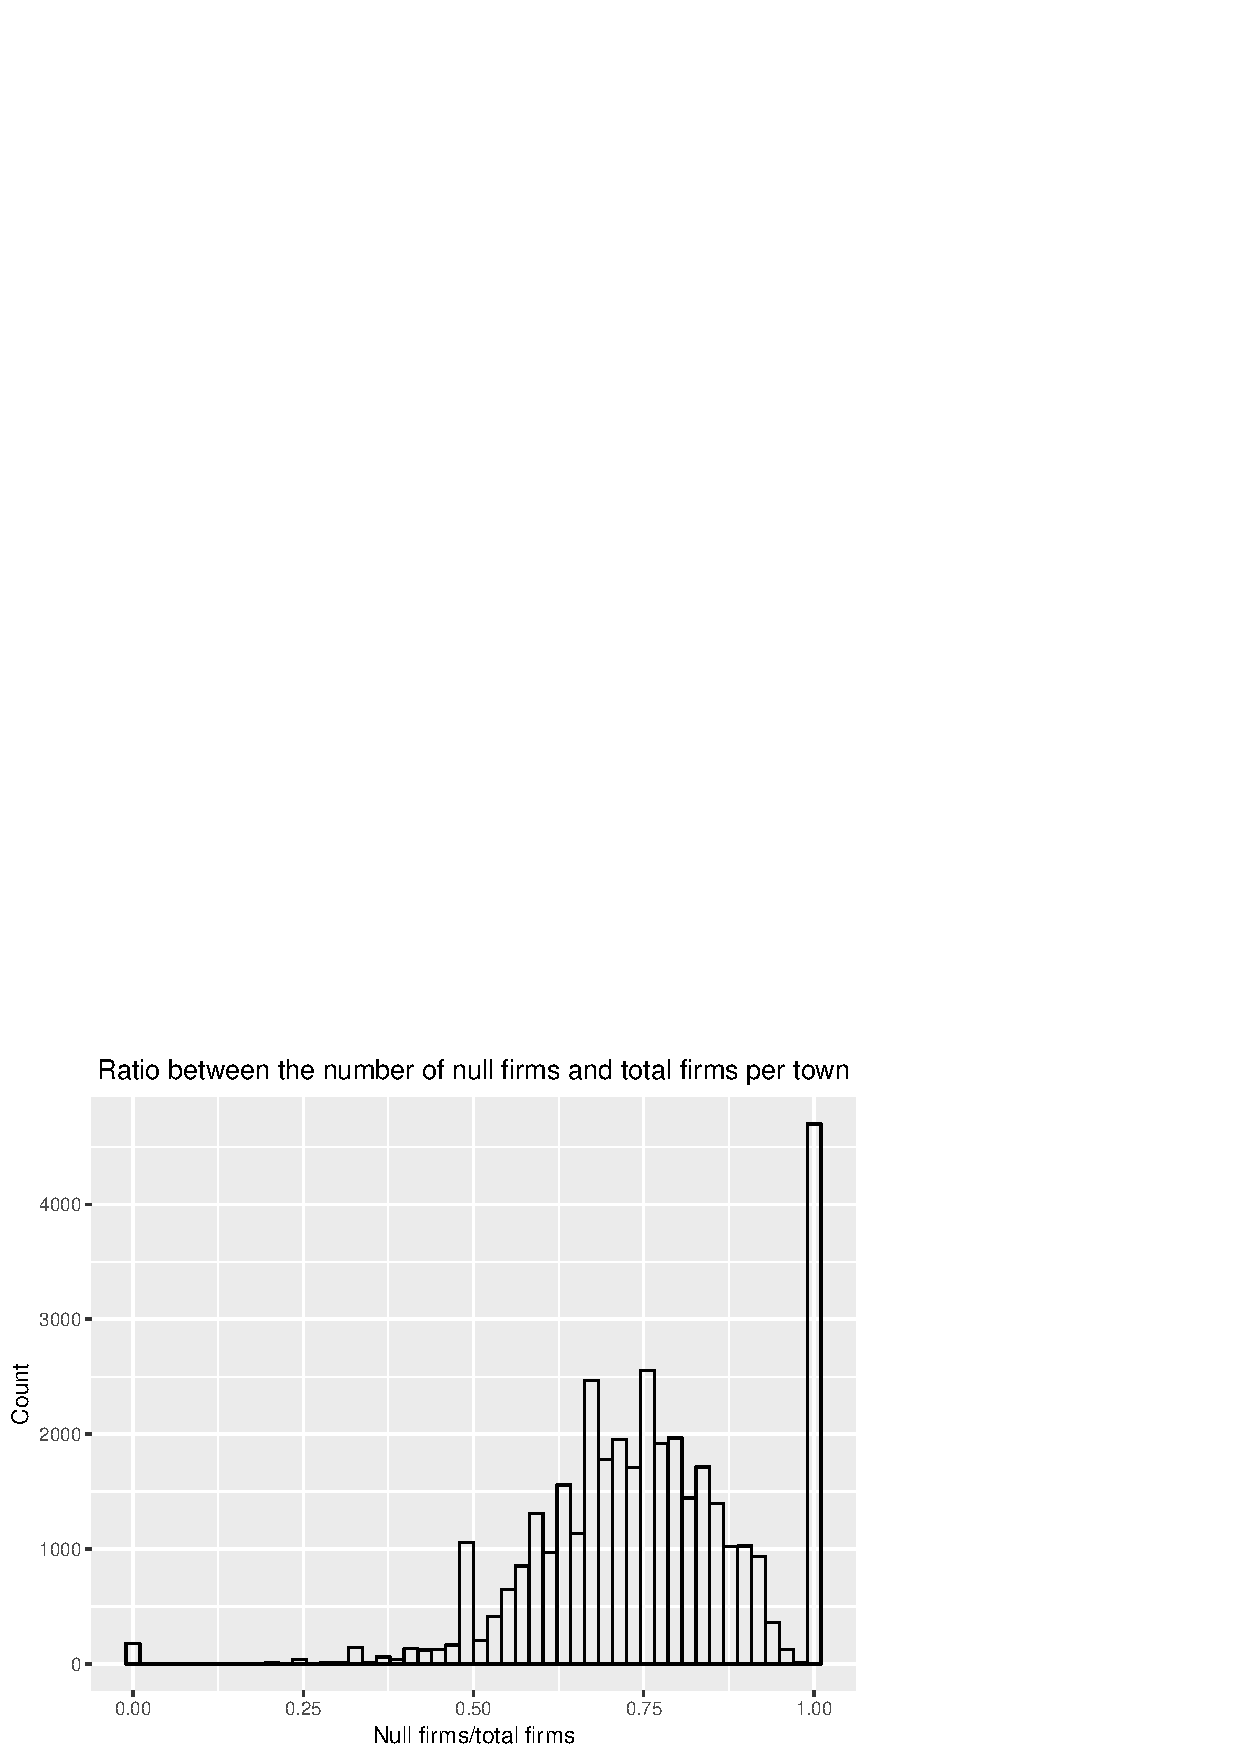
\includegraphics[width=0.5\textwidth]{hist_firms_ratio_null_total.jpeg}}
	\caption{} 
	\label{fig4}
\end{figure}
\end{frame}


\section{4. What has been done so far...}
	\begin{frame}{\vskip 0.05cm\centerline{\Huge\textcolor{bscuro}{What has been done so far \ldots}}}
	%	  State clearly what you were able to accomplish during the course, illustrate methods used and results.
		\begin{itemize}
			\item Geography:
			\begin{itemize}
				\item xx;
			\end{itemize}
		\end{itemize}
\end{frame}


\section{Issues}
		\begin{frame}{\vskip 0.05cm\centerline{\Huge\textcolor{bscuro}{Issues}}}

\end{frame}			
		

\section{Future works}
		\begin{frame}{\vskip 0.05cm\centerline{\Huge\textcolor{bscuro}{Future works}}}
%		Elaborate on future plans; can what you did during the course be the basis for a continuing project/collaboration? 
Combine the seperated dataset\\
how much less do women earn than men (for different department)? 
\end{frame}		
	
\section{End}
	\begin{frame}
	\centerline{\Huge\textcolor{bscuro}{ -- \emph{Thank you} -- }}
\end{frame}

\end{document}
